\newpage
\fancyhead[LH]{上海交通大学学位论文}
\fancyhead[RH]{第五章\quad 基于优化的路侧导航增强原理}
\section{基于优化的路侧导航增强原理}
为了提高对车辆的导航定位精度,有许多基于车载传感器的方案,例如视觉SLAM或激光SLAM。它们通过车辆对周边环境的观测,结合自身IMU/GNSS传感器的定位,用状态估计理论预测车辆位置。路侧单元对车辆的观测,本质与IMU,GNSS等传感器无异,也是观测量的一种。为了实现路端导航增强,我们需要将路侧观测考虑在传统的状态估计模型中。

\subsection{车辆状态估计的数学描述}
\label{sec5.1}
假设车辆装备着IMU,GNSS,相机等传感器在一个未知的环境里运动。由于传感器采样的时间是离散的,假设采样时刻为$t=1,2,...,k$。$x_t$为车辆在$t$时刻的位置\footnote[1]{这里为了简化模型,不同传感器的采样时刻假设为一致,现实中各传感器的时刻虽不一致,但不影响理论推导。},$X=\{x_1,x_2,...,x_k\}$为车辆的轨迹。车载传感器GNSS对自身速度的观测量为$G=\{g_1,g_2,...,g_k\}$。车载传感器IMU对自身速度的观测量为$U=\{u_1,u_2,...,u_k\}$。路侧单元在$t$时刻对车辆的观测为$o_t$,轨迹为$O={o_1,o_2,...o_t}$。我们的状态估计问题为,已知时刻$t=1,2,...,k$对应的车辆对自身的观测$U$和$G$,路侧单元对车辆的观测$O$,预测车辆位置$X$。这是一个最大后验估计问题MAP(Maximum a Posteriori Inference),其数学描述为
\begin{equation}
    X^{MAP} = \arg\max\limits_Xp(X|Z)
\end{equation}
其中$Z=\{G,U,O\}$是观测量的集合。

根据贝叶斯概率公式
\begin{equation}
    \begin{aligned}
        X^{MAP}
        &= \arg\max\limits_X\frac{p(Z|X)p(X)}{p(Z)}\\
        &= \arg\max\limits_Xp(Z|X)p(X)
    \end{aligned}
    \label{eq5.2}
\end{equation}
第三行是由于$Z$是已知的观测量,所以上式中的分母$p(Z)$不会对最大后延概率对应的状态值产生影响。

\subsection{基于因子图的状态估计理论}

利用条件概率公式,\eqref{eq5.2}可以继续分解为条件概率的乘积
\begin{equation}
    \begin{aligned}
        \phi(X)=p(X|Z)
        &\sim p(Z|X)p(X)\\
        &= p(x_1)\prod\limits_ip(x_{i}|x_{i-1},u_i)\prod\limits_ip(g_i|x_i)\prod\limits_ip(o_i|x_i)\\
        &= \phi_0(x_1)\prod\limits_i\phi_i(x_{i-1},x_i)\prod\limits_ig_i(x_i)\prod\limits_io_i(x_i)
    \end{aligned}
\end{equation}
其中,第二个等号用到了各个传感器间相互独立的假设,第三个等号使用了如下记号:
\begin{gather}
    \phi(X)=p(X|Z)\\
    \phi_0(x_1)=p(x_1)\\
    \phi_i(x_i,x_{i+1})=p(x_{i}|x_{i-1},u_i)\\
    g_i(x_i)=p(x_i|g_i)\\
    o_i(x_i)=p(x_i|o_i)
\end{gather}

这种将函数分解为乘积形式的写法可以进一步用因子图来描述,如图\ref{fig28}所示。图中包含了4种因子节点,先验节点$\phi_0$,运动模型节点$\phi_i$,和来自GNSS/RSU的观测节点\footnote[1]{本文定义的观测节点和SLAM里的观测节点概念不同,前者是环境(GNSS/RSU)对车辆的观测,后者是车辆对环境的观测。}$g_i$,$o_i$。

\begin{figure}[htb] 
    \center
    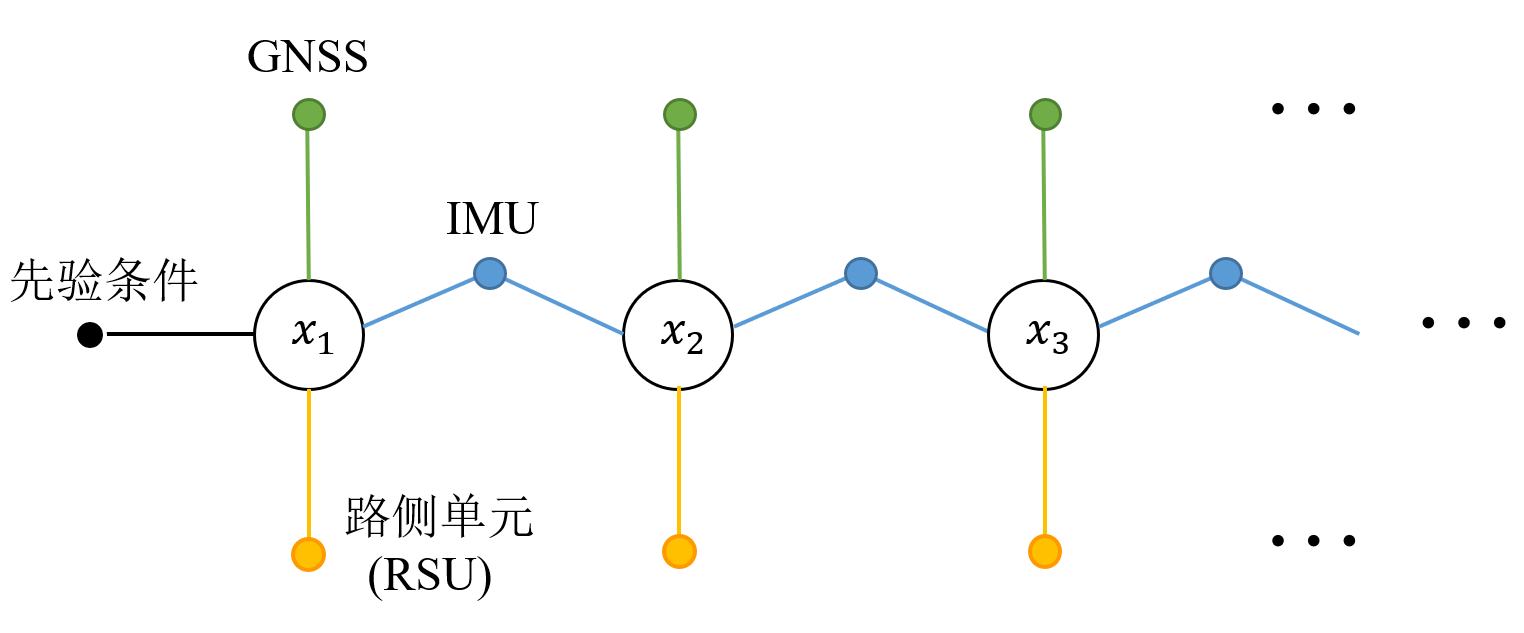
\includegraphics[width=0.8\textwidth]{figure/fig28.png}
    \caption{车辆估计的因子图描述}
    \label{fig28}
\end{figure}

假设每个因子对应的误差模型都满足零均值的多元高斯分布
\begin{equation}
    \begin{aligned}
        N(\theta;\mu,\Omega)&=\frac{1}{\sqrt{||2\pi\Omega||}}\exp\left\{-\frac{1}{2}||\theta-\mu||^2_\Omega\right\}\\
        &=\frac{1}{\sqrt{||2\pi\Omega||}}\exp\left\{-\frac{1}{2}||r||^2_\Omega\right\}\\
    \end{aligned}
\end{equation}
其中$\mu\in\mathbb{R}^n$是均值,$\Omega$是$n\times n$的协方差矩阵,$\theta$为分布的自变量,$r=||\theta-\mu||$为残差,
\begin{equation}
    ||\theta-\mu||^2_\Omega=(\theta-\mu)^T\Omega^{-1}(\theta-\mu)
\end{equation}
是马氏距离(Mahalanobis Distance)的平方。

求解原问题的最大后验概率分布等价于求该概率负对数的最小值。
\begin{equation}
    \begin{aligned}
        X^{MAP}&=\arg\max\limits_{X}p(X)\\
        &=\arg\max\limits_{X}\exp\left\{||r_{x_0}||_{\Omega_0}^2\right\}\prod\limits_i\exp\left\{||r_{x_i}||_{\Omega_i}^2+||r_{o_i}||_{R_i}^2+||r_{g_i}||_{Q_i}^2\right\}\\
        &=\arg\min\limits_{X}\left(||r_{x_i}||_{\Omega_i}^2+\sum\limits_i\left(||r_{x_i}||_{\Omega_i}^2+||r_{o_i}||_{R_i}^2+||r_{g_i}||_{Q_i}^2\right)\right)
    \end{aligned}
    \label{eq5.11}
\end{equation}
其中$r_{x_0}$,${r_{x_i}}$,$r_{g_i}$和$r_{o_i}$分别为先验模型,运动模型和来自GNSS/RSU的观测模型的残差项。

% \textbf{系统先验因子节点}
% 先验因子是因子图中的一个独立因子,该因子包含了系统的初始状态,为系统状态的迭代
% 求解奠定了基准。其残差可以表示为$r_{x_0}=$

\textbf{IMU因子节点}论文\cite{forster2016manifold}给出了一种IMU预积分算法。该算法可以计算因子图中两个节点间IMU测量值的预积分,为优化步骤提供高频率的状态更新。时刻$i-1$到时刻$i$间的残差定义如下:
\begin{equation}
    \mathbf{r}_{x_i}=[\mathbf{r}^T_{\Delta\mathbf{R}_i}, \mathbf{r}^T_{\Delta\mathbf{p}_i},\mathbf{r}^T_{\Delta\mathbf{v}_i}]^T\in\mathbb{R}^9
\end{equation}
其中,$\mathbf{r}^T_{\Delta\mathbf{R}_i}, \mathbf{r}^T_{\Delta\mathbf{p}_i},\mathbf{r}^T_{\Delta\mathbf{v}_i}$分别为来自姿态角$\mathbf{R}$(Rotation),位置$\mathbf{p}$(Pose)和速度$\mathbf{v}$(velocity)的残差项。\begin{equation}
    \begin{aligned}
        \mathbf{r}_{\Delta\mathbf{R}_i} &=\log\left(\Delta\tilde{\mathbf{R}}_{i}(\mathbf{b}_{i-1}^g)\right)\mathbf{R}_{i-1}^T\mathbf{R}_i  \\
        \mathbf{r}_{\Delta\mathbf{p}_i} &=\mathbf{R}_{i-1}^T\left(\mathbf{p}_i-\mathbf{p}_{i-1}-\mathbf{v}_{i-1}\Delta t_{\Delta i}-\frac{1}{2}\mathbf{g}\Delta t_{i}^2\right) -\Delta\tilde{\mathbf{p}}_{\Delta i}(\mathbf{b}_{i-1}^g,\mathbf{b}_{i-1}^a) \\
        \mathbf{r}_{\Delta\mathbf{v}_i} &=\mathbf{R}_{i-1}^T\left(\mathbf{v}_i-\mathbf{v}_{i-1}-\mathbf{g}\Delta t_{\Delta i}\right) -\Delta\tilde{\mathbf{v}}_{i}(\mathbf{b}^g_{i-1},\mathbf{b}^a_{i-1})  \\
        \mathbf{r}_{\Delta\mathbf{b}_i} &=\mathbf{b}_i-\mathbf{b}_{i-1} 
        \end{aligned}
\end{equation}
具体的推导可参见\hyperref[app1]{附录A}

\textbf{GNSS因子节点}可以表示为
\begin{equation}
    g_i(x_i)=\frac{1}{\sqrt{||2\pi R||}}\exp\left\{-\frac{1}{2}||h_g(x_i)-g_i||^2_R\right\}
\end{equation}
其中$h_g(X)$是高斯分布的均值,其现实意义为,当物体轨迹为$X$时,观测量$G$的理论值,$h_g$为测量函数,$R$为高斯分布的协方差矩阵。

\textbf{RSU因子节点}可以表示为
\begin{equation}
    o_i(x_i)=\frac{1}{\sqrt{||2\pi Q||}}\exp\left\{-\frac{1}{2}||h_o(x_i)-o_i||^2_Q\right\}
    \label{eq5.14}
\end{equation}
其中$h_o(X)$是高斯分布的均值,其现实意义为,当物体轨迹为$X$时,观测量$O$的理论值,$h_o$为测量函数,$Q$为高斯分布的协方差矩阵。

\subsection{基于因子图的非线性最优化算法}

在获得\eqref{eq5.11}后,问题被转化为了一个非线性优化问题。非线性问题的复杂度和困难度远大于线性问题。非线性函数含有高阶无穷小项,因此难以获得函数的所有解析解。但我们可以用线性化的方法,获得函数的局部最优解。以\eqref{eq5.14}为例,将其在$x_0$线性化可以将问题转化为
\begin{equation}
    \xi^*=\arg\min\limits_\xi||h_o(x_0)+\mathbf{J}_{x_0}\xi-o_i||^2_Q
    \label{eq5.16}
\end{equation}
传统的方法有梯度下降法,高斯牛顿法或列文伯格-马夸尔特(L-M)法等。

\textbf{梯度下降法}沿着梯度下降的方向进行优化计算,步长$\xi$计算如下
\begin{equation}
    \mathbf{J}_{x_0}\xi=o_i-h_o(x_0)\Rightarrow\xi=\lambda\mathbf{J}_{x_0}^T(o_i-h_o(x_0))
\end{equation}
其中$\lambda$是迭代系数,控制下降的速度。

\textbf{高斯牛顿法}计算了函数的二阶导数来拟合非线性函数。对\eqref{eq5.16}进行展开,获得误差函数的二阶翻书,求导可以得到极值点,从而获得扰动变量$\xi$的求解方程
\begin{equation}
    \mathbf{J}_{x_0}^T\mathbf{J}_{x_0}\xi=\mathbf{J}_{x_0}^T(o_i-h_o(x_0))
\end{equation}

\textbf{L-M算法}结合了梯度下降法和高斯牛顿算法,把迭代步长控制在一个范围内
\begin{equation}
    (\mathbf{J}_{x_0}^T\mathbf{J}_{x_0}+\lambda\mathbf{I})\xi=\mathbf{J}_{x_0}^T(o_i-h_o(x_0))
\end{equation}
$I$是单位矩阵,$\lambda$是调控系数,当$\lambda$比较大时,方法等价于梯度下降法,反之,当$\lambda$趋近于0时等价于高斯牛顿法。

此外,GTSAM\cite{dellaert2012factor}也被广泛用于非线性最优化问题。GTSAM是一种用于视觉SLAM和非线性优化的开源C++库。它是一种高效、通用的图优化框架,可以在多个领域中应用,包括机器人、无人机、自动驾驶汽车等。GTSAM支持多种传感器类型,例如相机、IMU、GPS等,并提供了基于因子图的概率推理框架,能够精确地估计状态变量,并根据测量数据进行更新优化。此外,GTSAM还提供了一组易于使用的API,使得使用者可以方便地构建SLAM系统,并加入自定义的因子模型。

\subsection{本章小结}
本章首先介绍了路侧增强的数学模型,再介绍了基于因子图的状态估计理论,各个因子节点的残差计算,最后介绍了因子图理论中的常用的优化方法。